\documentclass{anstrans}
%%%%%%%%%%%%%%%%%%%%%%%%%%%%%%%%%%%
\title{Residual Monte Carlo Treatment of the Time Variable with Consistent Acceleration for Thermal
Radiative Transfer Problems}
\author{Simon R.~Bolding and Jim E.~Morel}

\institute{Texas A\&M University Nuclear Engineering Department, 
}

\email{sbolding@tamu.edu \and morel@tamu.edu}

% Optional disclaimer: remove this command to hide
%\disclaimer{Notice: this manuscript is a work of fiction. Any resemblance to
%actual articles, living or dead, is purely coincidental.}

%%%% packages and definitions (optional)
\usepackage{graphicx} % allows inclusion of graphics
\usepackage{booktabs} % nice rules (thick lines) for tables
\usepackage{microtype} % improves typography for PDF
\usepackage{comment}
\usepackage{float}

\newcommand{\SN}{S$_N$}
\renewcommand{\vec}[1]{\bm{#1}} %vector is bold italic
\newcommand{\vd}{\bm{\cdot}} % slightly bold vector dot
\newcommand{\grad}{\vec{\nabla}} % gradient
\newcommand{\ud}{\mathop{}\!\mathrm{d}} % upright derivative symbol
\renewcommand{\eqref}[1]{(\ref{#1})}
\renewcommand*\thetable{\Roman{table}}
\usepackage{caption}

\captionsetup[table]{labelsep=period}
\captionsetup[figure]{labelsep=period}
\newcommand{\N}{\mathbb{N}}
\newcommand{\Z}{\mathbb{Z}}
\newcommand{\deriv}[2]{\frac{\mathrm{d} #1}{\mathrm{d} #2}}
\newcommand{\pderiv}[2]{\frac{\partial #1}{\partial #2}}
\newcommand{\bx}{\mathbf{X}}
\newcommand{\ba}{\mathbf{A}}
\newcommand{\by}{\mathbf{Y}}
\newcommand{\bj}{\mathbf{J}}
\newcommand{\bs}{\mathbf{s}}
\newcommand{\B}[1]{\ensuremath{\mathbf{#1}}}
\newcommand{\Dt}{\Delta t}
\renewcommand{\d}{\mathrm{d}}
\newcommand{\mom}[1]{\langle #1 \rangle}
\newcommand{\xl}{{x_{i-1/2}}}
\newcommand{\xr}{{x_{i+1/2}}}
\newcommand{\il}{{i-1/2}}
\newcommand{\ir}{{i+1/2}}
\newcommand{\keff}{\ensuremath{k_{\text{eff}}}}
\newcommand{\sig}[1]{\ensuremath{\Sigma_{#1}}}
\newcommand{\ra}{\ensuremath{\rightarrow}}
\newcommand{\dd}{\ensuremath{\mathrm{d}}}
\renewcommand{\O}{\ensuremath{\mathbf{\Omega}}}
\newcommand{\adj}{\ensuremath{{}^{\dagger}}}
\newcommand{\x}{\ensuremath{\mathbf{x}}}
\newcommand{\T}{\ensuremath{\text{T}}}
\newcommand{\iso}[2]{$^{#2}$#1}
\newcommand{\phibar}{\ensuremath{\overline{\phi}}}
\newcommand{\cur}[1]{\left\{ #1 \right\}}
\newcommand{\jl}{{j-1/2}}
\newcommand{\jr}{{j+1/2}}
\newcommand{\E}[1]{\ensuremath{\operatorname{E}_{#1}}}
\newcommand{\rface}{\ensuremath{r_{\text{face}}}}
\newcommand{\FOM}{\ensuremath{\text{FOM}}}
\newcommand{\ds}[0]{\displaystyle}
\newcommand{\invcm}[0]{cm$^{-1}$}
\renewcommand{\u}[1]{\ensuremath{\underline{#1}}}
\newcommand{\dep}{\ensuremath{\delta\epsilon^{(m)}}}
\renewcommand{\ss}{\ensuremath{\|s\|}}
\newcommand{\pos}{{\text{pos}}}
\newcommand{\phsp}{\ensuremath{\left(\mathbf{r},\mathbf{\Omega},\nu,t\right)}}
\newcommand{\Del}{\ensuremath{\nabla}}


\begin{document}
%%%%%%%%%%%%%%%%%%%%%%%%%%%%%%%%%%%%%%%%%%%%%%%%%%%%%%%%%%%%%%%%%%%%%%%%%%%%%%%%
\section{Introduction}

Accurate solution to the thermal radiative transfer (TRT) equations is important in the
high-energy, high-density physics regime, e.g., for inertial
confinement fusion and astrophysics simulations.  Moment-based hybrid Monte Carlo (MC)
methods have demonstrated great potential for accelerated
solutions to TRT problems.   Such methods iterate between a
high-order (HO) transport equation and a low-order (LO) system formulated with angular moments
of the transport equation over a fixed spatial mesh.  Physics operators that
are too expensive for the HO solver to resolve directly, e.g., photon absorption and emission,
are moved to the LO system. The lower-rank LO equations can be solved with Newton
methods to allow for non-linearities in the LO equations to be efficiently
resolved.  The high-order (HO) problem is defined by the transport equation
that models the photon radiation with sources defined by the previous LO solution. Solution to the HO
problem is used to construct consistency terms that require the next LO solution to be
consistent with the HO solution.  These consistency terms preserve the accuracy of the MC
solution method in the LO equations, upon nonlinear convergence of the outer iterations.

Previously, residual Monte Carlo (RMC) methods have been used to provide efficient
solution to the HO transport problem~\cite{rmc,bolding_nse}; high-fidelity solutions,
with minimal statistical noise, have been achieved for problems with optically-thick, diffusive
regions that lead to slowly varying
solutions.  However, the results in these works used a backward
Euler (BE) discretization for the time variable, which can inaccurately disperse radiation
wavefronts in optically thin problems. We have extended the work
in~\cite{bolding_nse} to include higher-accuracy treatment of the time variable for the
radiation unknowns. The exponentially-convergent Monte Carlo (ECMC)
algorithm~\cite{bolding_nse} was modified to include integration of the time variable;
this includes the introduction of a step, doubly-discontinuous (SDD) trial space representation
in time.  A new
parametric closure of the LO equations, introducing additional time-closure consistency
terms, was derived to capture the time accuracy of the HO
ECMC simulations.  The LO equations can preserve the accuracy of MC radiation transport treatment in
time, with the same numerical expense as Backward Euler (BE) time discretized S$_2$ equations. We have derived the LO equations directly from the transport equation,
such that, neglecting spatial discretization differences,
the HO and LO solutions are consistent upon convergence.
Herein we briefly describe the HO and LO solvers, and we preset results for
one-dimensional (1D), grey test problems.  We compare our method to the implicit MC
(IMC) method~\cite{wollaber_review}, the standard MC solution
method for TRT problems.

%%%%%%%%%%%%%%%%%%%%%%%%%%%%%%%%%%%%%%%%%%%%%%%%%%%%%%%%%%%%%%%%%%%%%%%%%%%%%%%%
\section{Theory}
The 1D, grey TRT equations consist of the radiation and
material energy balance equations, i.e.,\vspace{-0.05in}
\begin{align}\label{ho_cont}
    \frac{1}{c}\pderiv{I(x,\mu,t)}{t} + \mu \pderiv{I(x,\mu,t)}{x} &+ \sigma_a
    I(x,\mu,t)
= \frac{1}{2} \sigma_a a c T^4(x,t)
    \\ \label{t_cont}
  \rho c_v \pderiv{T(x,t)}{t} &=  \sigma_a \phi(x,t) - \sigma_a a c T^4(x,t),
\end{align}
where physical scattering could optionally be included in Eq.~\eqref{ho_cont}.
In the above equations $x$ is the position, $t$ is the time, $\mu$ is
the $x$-direction cosine of the angular intensity $I(x,\mu,t)$, $\sigma_a$ is the
macroscopic absorption cross section (cm$^{-1}$), and $a$, $c$, $\rho$,
and
$c_v$ are the radiation constant, speed of light, mass density, and specific heat,
respectively.  The desired transient unknowns are the material
temperature $T(x,t)$ and the mean radiation intensity $\phi(x,t)=\int_{-1}^1
I(x,\mu,t) \d \mu$.  The mean intensity is related to the radiation energy density
$E_r$ by the relation $E_r = \phi/c$.  The equations can be 
strongly coupled through the gray Planckian emission source $\sigma_a a c T^4$, which
is a nonlinear function of temperature, and the absorption
term $\sigma_a \phi$.   In general, the material properties are a function of $T$.  

In the HOLO context, the LO solver models the physical scattering and
resolves the material temperature spatial distribution $T(x)$ over each time step.  The HO solver
computes angular and temporal relations for $I$.  The
fully-discrete LO equations are based on algebraic manipulations of exact moment equations,
formed over a spatial finite-element (FE)
mesh.  The BE time discretization is applied to emission source throughout, but the radiation
variables are left in terms of time-averaged and end-of-time-step unknowns.  This is analagous to
the time-integration in IMC~\cite{wollaber_review}.   Angularly, the LO
radiation equations are similar to S$_2$ equations,  with element-averaged
consistency parameters that are weighted averages of $\mu$.  Additional
consistency parameters are introduced in a parametric closure that eliminates the auxillary
time-unknowns for radiation quantities.
If the angular and time
consistency parameters were estimated exactly, then the LO equations are exact moment equations,
neglecting spatial discretization error.  The consistency parameters are lagged
in each LO solve, estimated from the previous HO solution for $I(x,\mu,t)$,
as explained below. For the initial LO solve, within a time step, the angular parameters
are calculated based on the $I(x,\mu)$ from the previous time step and the LO equations use a standard time discretization.  The LO equations always conserve energy,
independent of the accuracy of the consistency terms.

The solution to the LO system is used to construct a spatially linear-discontinuous (LD) FE representation of
the emission source on the right hand side of Eq.~\eqref{ho_cont}.  This defines a fixed-source, pure absorber
transport problem for the HO operator. This HO transport problem represents a characteristic method that uses MC to
invert the continuous streaming plus removal operator with an LD representation of
sources. We will solve this transport problem using the ECMC algorithm.  The ECMC algorithm uses
batches of MC histories to estimate the error in the current trial-space representation of the
$I(x,\mu,t)$.  Because we are not using
mesh adaptation, exponential convergence in iterations cannot be maintained, but the benefit of residual MC can
still be achieved.  The output from ECMC is a projection $\tilde I(x,\mu,t)$ of the intensity onto
the chosen trial space. This projection will accurately resolve the end-of-time step intensity. Once computed, $\tilde{I}(x,\mu)$ is used to directly evaluate the
necessary LO angular consistency parameters and the time closure.   The HO solution is not used to directly estimate a new temperature at
the end of the time step; it is only used to estimate the parameters that go into the LO
equations, which eliminates typical operator splitting stability issues that require linearization of
the emission source.

The process of performing subsequential HO and LO solves occurs within a single time step, can
be repeated to obtain an increasingly accurate solution for $\phi^{n+1}(x)$ and
$T^{n+1}(x)$. However, for the problems tested here, only a single HO solve is performed during each
time step.  Thus, the HOLO algorithm, for the $n$-th time step, is

\begin{enumerate}
    \item Perform a LO solve to produce an initial guess for $T_{LO}^{n+1}(x)$
        and $\phi_{LO}^{n+1}(x)$, based on consistency terms estimated with $\tilde{I}^{n}$ and a BE time
    discretization.
\item Solve the HO system for $\tilde{I}_{HO}^{n+1}(x,\mu,t)$ using ECMC, based on the current
    LO estimate of the emission and scattering sources.%$\sigma_s(T^k)\phi^{k}$ and $B(T)^{k}$.
\item Compute LO consistency parameters with $\tilde{I}_{HO}^{n+1}$.  
\item Solve the LO system using HO consistency parameters to produce a new
    estimate of $\phi^{n+1}_{LO}$ and $T^{n+1}_{LO}$.
\item Store $\tilde{I}^{n}\leftarrow\tilde{I}^{n+1}$, and move to the next time step.
\end{enumerate}
where the superscript $k$ denotes an outer HOLO iteration.
The convergence criteria is based on successive LO solutions for $\phi^{n+1}(x)$ and
$T^{n+1}(x)$. The consistency terms force the HO
and LO solutions for $\phi^{n+1}(x)$ to be consistent to the order of the current HOLO
iteration error.

\subsection*{The LO System}
\label{sec:lo}

To derive the LO equations, we reduce the dimensionality of Eq.~\eqref{ho_cont} and
Eq.~\eqref{t_cont} by taking spatial, angular, and
temporal integrals.  The spatial moments are taken over each spatial cell $i$:
$x\in[x_{i-1/2},x_{i+1/2}]$, weighted with standard linear finite element basis functions.  For example, the left moment operator is defined by
\begin{equation}\label{x_mom}
\mom{\cdot}_{L,i} = \frac{2}{h_i} \int_{x_{i-1/2}}^{\xr} b_L(x) (\cdot) \d x,
\end{equation}
where $h_i=x_{i+1/2}-x_{i-1/2}$ is the width of the spatial element and
$b_L(x)=(x_{i+1/2}-x)/h_i$ is the FE basis function corresponding to position
$x_{i-1/2}$. Angularly, the equations are integrated over the positive and negative half-range integrals of the equations.
The angular integrals of the intensity are defined as $\phi^\pm(x) = \pm2\pi \int_0^{\pm 1} \psi(x,\mu) \d \mu$. 
Thus, in terms of half-range quantities, $\phi(x) = \phi^-(x) + \phi ^+(x)$.  Finally, the
equations are integrated over the $n$'th time step $t\in[t^n,t^{n+1}]$.  


For brevity, we now focus on the derivation of the new time treatment.  More specifics can be found in
literature~\cite{wolters,bolding_nse}.  The $+$ integral, $\mom{\cdot}_L$ moment, and
integration over a time step are applied to Eq.~\eqref{ho_cont}.
ultimately yields four
equations, for each cell.  Due to space limitations, only the final form of one
equation is given for reference as Eq.~\eqref{lo_eq} in the appendix.  The four
degrees of freedom (DOF) over each cell $i$ are $\mom{\phi}_{L,i}^+$,
$\mom{\phi}_{R,i}^+$, $\mom{\phi}_{L,i}^-$, and $\mom{\phi}_{R,i}^-$.  
The angular consistency terms are defined by the half-range averages
\begin{equation}\label{const}
\mom{{\mu}}_{L,i}^+ =  \frac{
{\displaystyle \frac{2}{h_i}} \int\limits_0^1 \int\limits_\xl^\xr \mu \, b_L(x)
\psi(x,\mu) \d x \d \mu } 
{{\displaystyle \frac{2}{h_i}} \int\limits_0^1 \int\limits_\xl^\xr \, b_L(x)
\psi(x,\mu) \d x \d \mu } .
\end{equation}
The consistency terms for the $R$ basis moment and $\mu_{i\pm1/2}^\pm$ face
terms are defined similarly.


The four coupled equations over each cell for the four DOF are exact; they have not been discretized
in any way.  However, the consistency parameters (defined by Eq.~\eqref{const}) are not known a priori, and
there is no relation between the volume and face averaged quantities.  In the HOLO
context, the equations for unknowns at iteration $m+1$ use consistency parameters
computed using Eq.~\eqref{const} and the latest HO solution $\tilde{\psi}^{m+1/2}$. For the initial LO
solve, all average $\mu$ parameters are
set to $\pm 1/\sqrt{3}$, yielding a solution equivalent to diffusion
with Mark boundary conditions (i.e., an S$_2$ solution).  To close the LO system spatially, the usual LD upwinding
approximation is used, which is consistent with the HO solution.  For example, for Eq.~\eqref{lo_eq}, the face terms $\mu_{i-1/2}$ and $\phi_{i-1/2}$
terms are upwinded from the previous cell $i-1$ (or boundary condition); the terms
at $x_{i+1/2}$ are linearly extrapolated, computed using the $L$ and $R$ basis moments.
  

Summing the equations over all cells, the global LO eigenvalue problem is formed.  In
operator notation, the global system is 
\begin{equation}\label{lo_k}
    \B D \Phi = \frac{1}{\keff} \B F \Phi,
\end{equation}
where $\Phi$ is the vector of unknown space-angle moments, $\B D$ represents
streaming plus removal minus scattering, and $\B F \Phi$ is the
fission source.  The matrix $\B D$ is an asymmetric banded matrix with a bandwith of
seven, which can
be directly inverted efficiently
without need for inner source iterations.  Eq.~\eqref{lo_k} is solved using inverse
power iteration, i.e., given $\keff^{(0)}$ and $\Phi^{(0)}$,
\begin{align*}
    \Phi^{(l+1)} = \frac{1}{\keff^{(l)}} \B D^{-1} \B F \Phi^{(l)}, &
    \quad \keff^{(l+1)} = \keff^{(l)}\frac{ \int \nu \sig f \phi^{(l+1)} \d
    x}{ \int \nu \sig f \phi^{(l)}\d x }.
\end{align*}
The $l$ iteration indices here are independent of the HOLO iteration $m$.
The above power iteration is repeated until $\keff^{(l)}$ and $\B F \Phi^{(l)}$ are
converged.  


\subsection*{The ECMC High Order Solver}

The transport equation to be solved by ECMC is given by Eq.~\eqref{ho_trans}. 
For the HOLO context, in operator notation, this equation is defined as
\begin{equation}\label{te_oper}
\B L I^{m+1/2}  = q^{m}
\end{equation}
where $I^{m+1/2}$ is the intensity based on the $m$-th
LO estimate of $q$, which is the Planckian emission source using $T^{n+1,m}$.  The \emph{continuous} linear operator $\B L$ includes the streaming, removal, and
time derivative on the left-hand side of Eq.~\eqref{ho_trans}.  

To perform the residual MC algorithm, it is necessary to have a trial space representation
of the solution over all of the phase space.  The intensity is represented in $x$ and $\mu$ with a
standard LDFE representation~\cite{bolding_nse}.  A step, doubly-discontinuous (SDD) trial
space is used to represent the intensity as a function of time.  The trial space
representation for $I(x,\mu,t)$ is then
\begin{equation}\label{eq:time_space}
    \tilde I(x,\mu,t) = \left \{ \begin{array}{cl}
        \tilde I^{n}(x,\mu)  & \quad t = t^n \\ 
        \overline I(x,\mu)  & \quad t \in (t^{n},t^{n+1}) \\               
      \tilde I^{n+1}(x,\mu)   &  \quad        t = t^{n+1}
    \end{array}           \right.
\end{equation}
where we have used $\overline I$ to denote the time-averaged LDFE \emph{projection} in $x$
and $\mu$ of the intensity over the interior of the time step;  the beginning and end of
time step projections are denoted $\tilde I^{n}$ and $\tilde I^{n+1}$, respectively.    
There is a projection error in using the LDFE projection to represent the intensity between time steps.  However, with
sufficient noise reduction and mesh resolution, this should be an acceptable error
compared to the large statistical noise of standard MC. The SDD trial space provides a
projection for all the desired unknowns that result from time-integration of the transport
equation to produce a balance equation, i.e., the time-averaged, end of time step, and
previous time step intensities. Another benefit of this
trial space is it allows for infrastructure for computing the residual from the
time-discrete case analytically to be used directly.  

To define the ECMC algorithm, the HOLO iteration indices
$m$ are dropped, noting that the LO estimated $q^{m}$ remains constant over the entire HO solve.
The $i$-th approximate solution to Eq.~\eqref{te_oper} is $\tilde{I}^{(i)}$, where
$i$ identifies the MC batch.
The $i$-th residual is $r^{(i)} = q - \B L\tilde{\psi}^{(i)}$, which with manipulation gives the error equation
\begin{equation}
\B L (\psi - \tilde{\psi}^{(i)}) = \B L \tilde{\epsilon}^{(i)} = r^{(i)}
\end{equation}
where $\psi$ is the exact solution and $\tilde{\epsilon}^{(i)}$ is finite element
representation, in space and angle, of the error in
$\tilde{\psi}^{(i)}$. The above equation represents a second, fixed-source, pure
absorber transport equation.
The operator $\B L$ is inverted without discretization via MC to produce an
estimate of the error in $\tilde{\psi}^{(i)}$, i.e., $\tilde{\epsilon}^{(i)} = \B
L^{-1} r^{(i)}$.
The projections of $\epsilon$ and $\psi$ onto the LD space-angle trial space are computed using standard
volumetric path-length
estimators.  A generalization to the linear basis functions for tallies used to estimate census energy from IMC~\cite{wollaber_review}.  The estimators are weighted by appropriate basis functions 
to tally the zeroth and first moments, in $x$ and $\mu$, of 
$I(x,\mu)$ over each space-angle cell.

  The ECMC algorithm is
\begin{enumerate}
\item Solve Eq.~\eqref{te_oper} to compute the MC projection of the angular
flux onto the LD $x-\mu$ trial space $\tilde\psi^{(0)}$.
\item Compute $r^{(i)}$.
\item Solve $\tilde{\epsilon}^{(i)} = \B L^{-1} r^{(i)}$
\item Compute $\tilde\psi^{(i+1)} = \tilde\psi^{(i)}
+ \tilde\epsilon^{(i)}$
\item Repeat 2 -- 4 until desired convergence of the angular flux is achieved.
\end{enumerate}

Convergence is based on the estimated relative error in $\tilde \psi^{(i)}$, defined as
$\epsilon_{rel} = \| \tilde \epsilon^{(i)} \|_2/\| \psi^{(0)} \|_2$.
Exponential convergence (with respect to the number
of particles simulated) of $\tilde \epsilon$ is obtained because with each inversion of $\B L$ a
more accurate estimate of the solution is used to compute the new residual, decreasing
the magnitude of the MC source $r^{(i)}$.  If the statistical estimate of $\tilde\epsilon$ is not sufficiently
accurate, then the batches would diverge.
Because the true angular flux does not in general lie within the LD trial space, the
iterative estimates of the error will eventually stagnate.  An adaptive $h-$refinement algorithm is used
to allow the system to continue converging towards the exact solution. 
Because some regions of refined cells are relatively small, the probability of particles being
sampled from those cells is very low.  To resolve issues this causes, stratified sampling is
used to sample the same number of source particles from each space-angle cell.  
Currently, the number of particles sampled
in each cell remains constant throughout the HO solve.

%%%%%%%%%%%%%%%%%%%%%%%%%%%%%%%%%%%%%%%%%%%%%%%%%%%%%%%%%%%%%%%%%%%%%%%%%%%%%%%%
\section{Results and Analysis}

We have simulated the following 1D, grey test problems to demonstrate the accuracy of the HOLO
algorithm: a thin problem and a standard Marshak wave. 
We use the L$_2$ measure of variance in the end of time step intensities to
form a figure of merit as

\subsection{Optically Thin Problem}

We modify the problem in the previous problem by increasing the absorption cross section to 0.2
\invcm; all other problem parameters are the same.  Radiation temperatures at the end of
the last time step are compared for IMC, HOLO-TC, and HOLO-BE in
Fig.~\ref{fig:thin_temp_compare}.  The HOLO-TC and HOLO-BE results were generated with 30
$\mu$ cells, and all spatial meshes used 200 cells.  At smaller time step sizes, the
effects of mesh imprinting are slightly apparent in the HOLO-TC results, leading to more
dispersion near the wave-front.  For $\Delta t=0.005$ sh, there is good agreement between
the HOLO-TC results and IMC.  As in the previous problem, the HOLO-BE results do not accurately capture
the wavefront location. IMC demonstrates substantial statistical noise in the equilibrium region.

\begin{figure}[H]
  \centering
    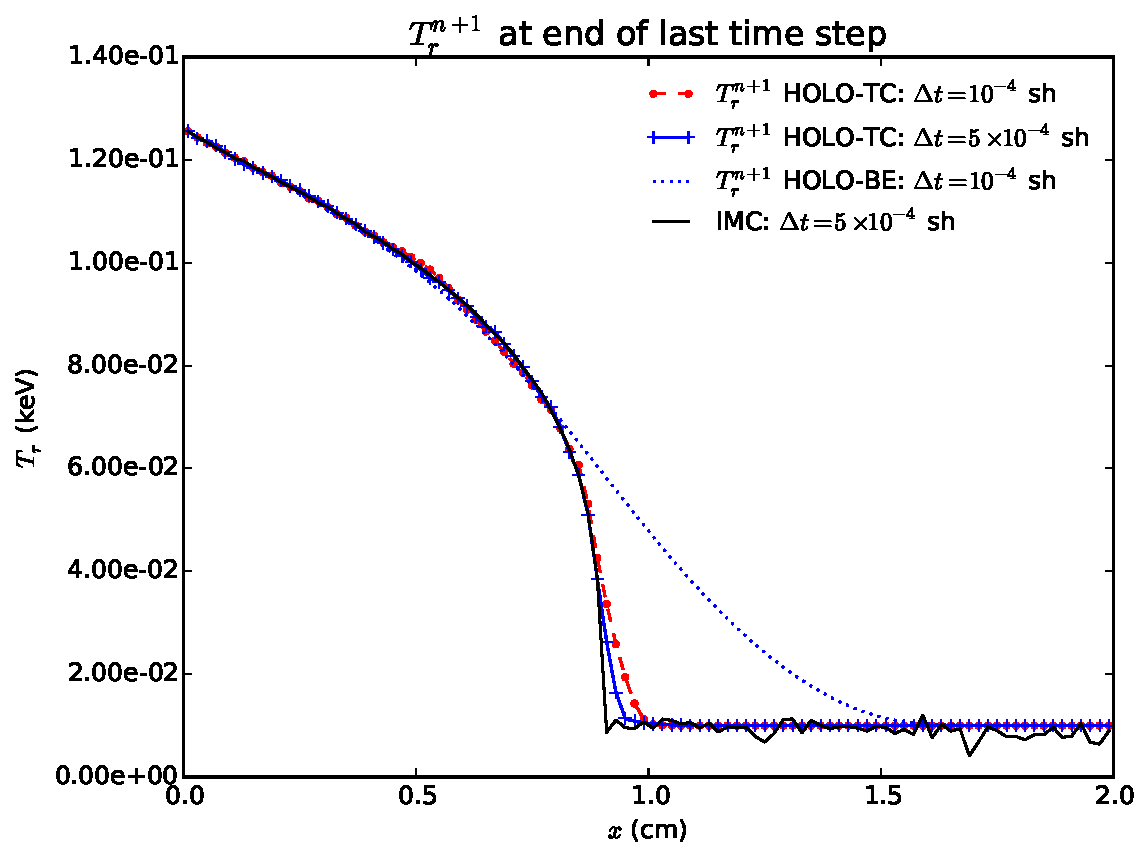
\includegraphics[width=0.75\textwidth]{thin_temp_compare.pdf}
    \caption{\label{fig:thin_temp_compare} Comparison of radiation temperatures of IMC and
    the HOLO method for different time step sizes and numbers of batches, for optically
thin problem. }
\end{figure}

Table.~\ref{tab:fom_thin} compares computed FOM values for the census
radiation energy densities, for the case of $\Delta t =
0.0005$~sh.  HOLO results were generated for the case of 1 and 2 batches, with the same
total number of histories per time step.  At low particle counts for the larger time step
size, the HOLO-TC method
demonstrates substantial noise.  This is due to the trial space representation of the
census particles at the end of the time step being poorly estimated.  For the 2 batch
case, the estimate from the first batch leads to less error in the census estimate as the
ECMC solves are simply solving for the deviation from the time-averaged quantity.  The
results for the case of 30,000 histories are plotted in Fig.~\ref{} for the HO and LO
solution.  As demonstrated, there seems to have been some instabilities introduced into
the LO equations through noise; sufficient sampling of the census must occur.
At smaller time-steps there is an increase in statistical efficiency, however there has
been a loss in accuracy due to an increase in projection error.  In general, this is a
balance that much be considered.

The accuracy of the HOLO-ECMC method was compared to a reference solution from IMC. This
problem is thin enough that we expect IMC to be accuracy with sufficient particle
histories.  The
reference solution is the average of 20 IMC simulations of $20\times10^6$
histories, each with $\delta t =10^{-4}$ sh.  The estimated value of $\ss$ for the
reference solution is 0.025\%.  The L$_2$ norm of the error in cell-averaged mean
intensities is computed 
at the end of the last time step, was computed.  The average over 20 simulations is then
computed to provide the metric
\begin{equation}
    \|e\|^l = \left({\frac{\sum\limits_{i=1}^{N_c}
    \left(\phi_i^{n+1,l} - \phi_i^{n+1,ref}
\right)^2}{\sum\limits_{i=1}^{N_c}\left(\phi_i^{n+1,ref}\right)^2}}\right)^{1/2},
\end{equation}
where $\phi_i^{n+1,l}$ is the cell-averaged scalar intensity at the end of the last time
step from the $l$-th independent simulation.  The sample mean of $\|e\|$ from 20
independent simulations provides a metric for the accuracy of a particular simulation:
\begin{equation}
    \overline{\|e\|} = \frac{1}{20}\sum_{l=1}^{20} \|e\|^l
\end{equation}

The accuracy results for 

\begin{table}[H]
\centering
\caption{\label{tab:void_short} {Comparison of sample statistics for the
    end of time step radiation energy densities, of the last time step, for the optically
    thin problem and $\Delta t = 5\times 10^{-4}$ sh.   Simulation end time is $\mathbf{t=0.003}$ sh.}}
\vspace{-0.1in}
\begin{tabular}{|c|ccc|ccc|}\cline{2-7}
    \multicolumn{1}{c|}{}       & \multicolumn{3}{|c|}{\ss} &
    \multicolumn{3}{|c|}{\FOM} \\ \hline
hists./step   & IMC & HOLO-TC (1) & HOLO-TC (3) &  IMC   & HOLO-TC(1) & HOLO-TC(3) \\ \hline
   30,000     & 3.01\%  & 18.29\% & 5.38\%      &  1.00  & 0.03  &  0.31      \\
  300,000     & 0.99\%  & 0.81\%  & 0.74\%      &  0.93  & 1.38  &  1.65     \\ 
  1,000,000   & 0.50\%  & 0.30\%  & 0.37\%      &  1.10  & 3.42  &  2.0      \\ \hline
\end{tabular}
\end{table}

\begin{table}[H]
\centering
\caption{\label{tab:void_short} {Comparison of sample statistics for the
    end of time step radiation energy densities, of the last time step, for the optically
    thin problem and $\Delta t = 1\times 10^{-4}$ sh.   Simulation end time is $\mathbf{t=0.003}$ sh.}}
\vspace{-0.1in}
\begin{tabular}{|c|ccc|ccc|}\cline{2-7}
    \multicolumn{1}{c|}{}       & \multicolumn{3}{|c|}{\ss} &
    \multicolumn{3}{|c|}{\FOM} \\ \hline
hists./step   & IMC & HOLO-TC (1) & HOLO-TC (3) &  IMC   & HOLO-TC(1) & HOLO-TC(3) \\ \hline
   30,000     & 3.00\%  & 0.55\% & 1.28\%       &  1.00  &  29.81    & 5.51    \\
  300,000     & 0.96\%  & 0.11\% & 0.30\%       &  0.98  &  71.82    & 9.88    \\ 
  1,000,000   & 0.49\%  & 0.06\% & 0.17\%       &  1.11  &  71.02    & 9.71    \\ \hline
\end{tabular}
\end{table}


\subsection{Marshak Wave Problem}

It is important to demonstrate that the time closures are stable in a mix of optically
thick and optically thin regions, and that the ECMC method is still efficient in such
problems.  Simulations were performed for the Marshak wave problem defined in
Sec.~\ref{sec:marshak}.  The time step size is linearly increased from $0.001$ sh to a
maximum step of 0.01 sh over the first 10 time steps; the last time step is adjusted to
reach the desired simulation end time.  It was found for this problem that it was
necessary to use more than one batch for the HOLO-TC algorithm to stably converge.
This is because in the case of a single batch particles must reach
census to accurately estimate the next time step value.  These results were generated using the implicit-like time
closure.

\begin{figure}[H]
    \centering
    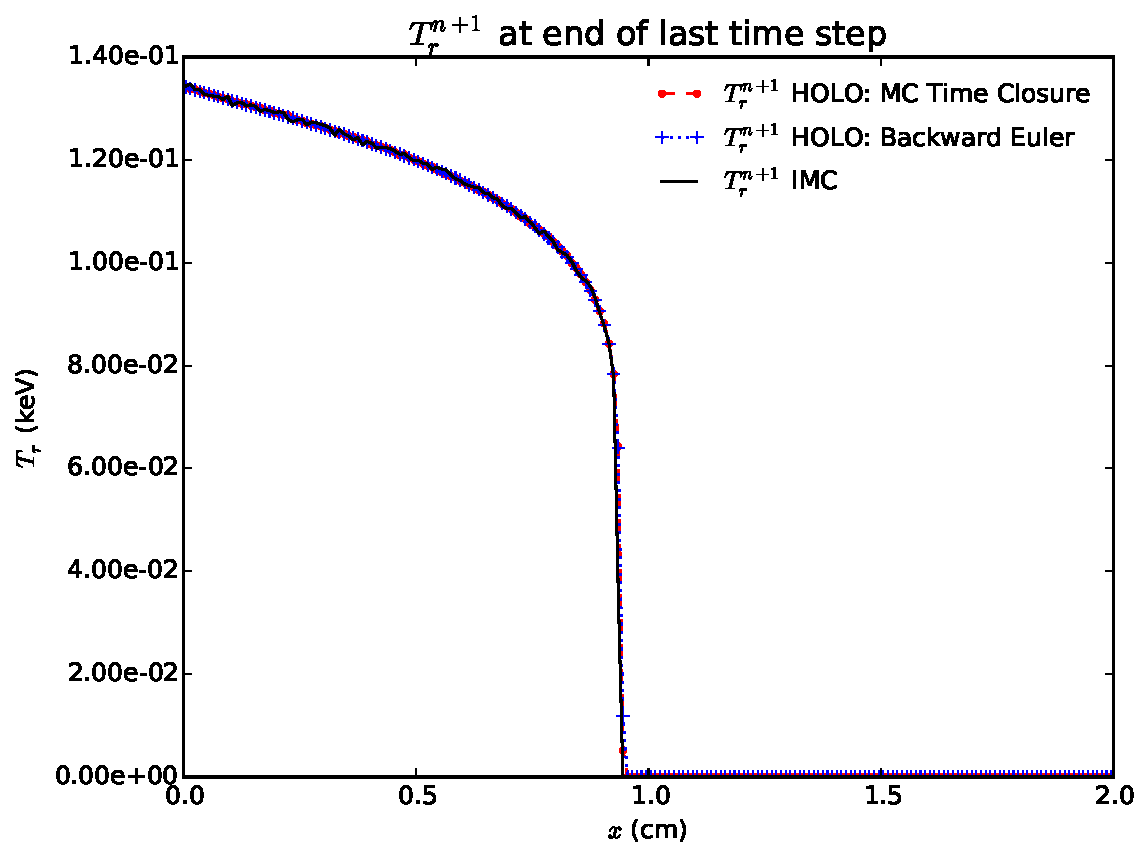
\includegraphics[width=0.65\textwidth]{marshak_time_cont_compare.pdf}
    \caption{\label{fig:marshak_tc} Comparison of HOLO-TC, HOLO-BE, and IMC methods for
the Marshak Wave problem, with $10^6$ histories per time step.}
\end{figure}

Figure~\ref{fig:marshak_tc} compares the accuracy of IMC, HOLO-TC, and HOLO-BE.  The
solutions are plotted at $t=3$ sh, with $10^6$ histories per time step for all
simulations. As demonstrated, there is good agreement among the results.  It is noted that
this problem can be accurately modeled with the Backward Euler time discretization, but
the MC time closure appears to be stable even in the mix of optically thick and thin
regions. Table~\ref{tab:marshak_cont} compares sample statistics for IMC and
the HOLO method with continuous time treatment and with a BE discretization.  As
demonstrated, at the lower history count (300,000), the HOLO-TC algorithm demostrates a
greater variance.  These results used the implicit
like time closure.

\begin{table}[H]
\centering
\caption{\label{tab:marshak_cont} {Comparison of sample statistics for the
    end of time step radiation energy densities, of the last time step, for the marshak
    wave problem and maximum time step of $0.01$ sh.  Simulation end time is $\mathbf{t=3.0}$ sh.}}
\vspace{-0.1in}
\begin{tabular}{|c|ccc|ccc|}\cline{2-7}
    \multicolumn{1}{c|}{}       & \multicolumn{3}{|c|}{\ss} &
    \multicolumn{3}{|c|}{\FOM} \\ \hline
hists./step   & IMC & HOLO-TC (2) & HOLO-BE (2) &  IMC   & HOLO-TC (2) & HOLO-BE (2) \\ \hline
  300,000     & 2.25\%  & 3.42\% & 0.30\%       &  1.00  &   0.43    & 2050          \\  
  1,000,000   & 1.27\%  & 0.31\% & 0.17\%       &  0.94  &  15.95    & 1806          \\ \hline
  \multicolumn{7}{|c|}{Diamond Like Closure} \\ \hline
  300,000     & --  & 3.53\% & --   &  --  &   0.41   & --  \\  
  1,000,000   & --  & 0.37\% & --   &  --  &  10.94   & --  \\ \hline
\end{tabular}
\end{table}




Later on, we can include a table, even one that spans two columns such as
Table~\ref{tab:widetable}.
%%%%%%%%%%%%%%%%%%%%%%%%%%%%%%%%%%%%%%%%
\begin{table*}[htb]
  \centering
\begin{tabular}{llllllllll}\toprule
      & $\phi_T(0)$      & $\phi_T(10)$      & $\phi_T(20)$      &
      $\phi_D(0)$      & $\phi_D(10)$      & $\phi_D(20)$      & $\rho$      &
      $\varepsilon$      & $N_\text{it}$
\\ \midrule
$c=0.999$  & 0.9038 & 20.63 & 31.24 & 0.9087 & 20.63 & 31.23 & 0.2192 & $10^{-7}$ & 15
\\
$c=0.990$  & 0.3675 & 13.04 & 24.7 & 0.3696 & 13.04 & 24.69 & 0.2184 & $10^{-7}$ & 15
\\
$c=0.900$  & 0.009909 & 4.776 & 17.64 & 0.009984 & 4.786 & 17.63 & 0.2118 & $10^{-7}$ & 14
\\
$c=0.500$  & $6.069\times 10^{-5}$ & 2.212 & 15.53 & 6.213$\times 10^{-5}$ & 2.239 & 15.53 & 0.2068 & $10^{-7}$ & 13
\\
\bottomrule
\end{tabular}
  \caption{This is an example of a really wide table which might not normally
  fit in the document.}
  \label{tab:widetable}
\end{table*}


%%%%%%%%%%%%%%%%%%%%%%%%%%%%%%%%%%%%%%%%%%%%%%%%%%%%%%%%%%%%%%%%%%%%%%%%%%%%%%%%
\section{Conclusions}



We believe that the doubly discontinuous trial space for the time variable suffers from the fact that you need a
point-wise estimate of the flux in the time variable.  Alternatively, the LDFE trial space
could also include the time variable (i.e., it is linear in time).  This has the added
benefit that the slope can be estimated over the interior of the time-step, so all
particle tracks contribute to the score.  However, there is some additional truncation
error as the end of time-step is an extrapolated quantity.  We are investigating the use
of the LD trial space, but it requires significant modifications to the sampling
algorithm; these modifications will be required to extend to higher spatial dimensions, so
they should provide an interesting tool.  We plan to include results for the LD representation in time for the full paper.



%%%%%%%%%%%%%%%%%%%%%%%%%%%%%%%%%%%%%%%%%%%%%%%%%%%%%%%%%%%%%%%%%%%%%%%%%%%%%%%%
\appendix
\section{Appendix}

Numbering in the appendix is different:
\begin{equation} \label{eq:appendix}
  2 + 2 = 5\,.
\end{equation}
and another equation:
\begin{equation} \label{eq:appendix2}
  a + b = c\,.
\end{equation}

%%%%%%%%%%%%%%%%%%%%%%%%%%%%%%%%%%%%%%%%%%%%%%%%%%%%%%%%%%%%%%%%%%%%%%%%%%%%%%%%
\section{Acknowledgments}

%%%%%%%%%%%%%%%%%%%%%%%%%%%%%%%%%%%%%%%%%%%%%%%%%%%%%%%%%%%%%%%%%%%%%%%%%%%%%%%%
\bibliographystyle{ans}
\bibliography{references}
\end{document}

